\documentclass[12pt,a4paper,titlepage]{article}
\usepackage[utf8]{inputenc}
\usepackage[german]{babel}
\usepackage{amsmath}
\usepackage{amsfonts}
\usepackage{amssymb}
\usepackage{setspace}
\usepackage{graphicx} %Um Bilder anzeigen zu können
\usepackage[top=1in, bottom=1.5in, left=1in, right=1in]{geometry}
\usepackage{endnotes}
\usepackage[section]{placeins}
\usepackage{fancyhdr}

\newcommand{\myma}{\fontfamily{pcr}\selectfont \textbf}
\newcommand{\mymo}{\fontfamily{pcr}\selectfont \textit}
\setlength{\parindent}{0pt}
\let\footnote=\endnote

\begin{document}
\pagestyle{fancy}

\begin{titlepage}
\vspace*{50pt}
\begin{center}
{\Huge Entwurf\\[1cm] {\bfseries Praxis der Softwareentwicklung}\\[2cm] Entwicklung einer Software zur Berechnung der Mandatsverteilung im Deutschen Bundestag\\[1cm]Gruppe 1} \\
\vspace*{15pt}
{\normalsize Philipp Löwer, Anton Mehlmann, Manuel Olk, Enes Ördek, \\Simon Schürg, Nick Vlasoff}
\end{center}
\date{}

\vspace*{30pt}
\begin{figure}[h]
\centering
		
\includegraphics[scale=0.6]{KIT-Logo.png}\\
		\vspace*{10pt}
		\Huge WS 2013 / 14
\end{figure}
\end{titlepage}
\newpage\thispagestyle{empty}\hspace{1em}\newpage
\def\Vhrulefill{\leavevmode\leaders\hrule height 0.7ex depth \dimexpr0.4pt-0.7ex\hfill\kern0pt}
\cfoot{{\Vhrulefill~  Seite \thepage   ~\Vhrulefill} \newline {\scriptsize KIT – Universität des Landes Baden-Württemberg und nationales Forschungszentrum in der Helmholtz-Gemeinschaft}}

\pagenumbering{roman} 

 
\newpage
\begin{onehalfspace}
\tableofcontents
\end{onehalfspace}
\newpage

\pagenumbering{arabic} 


\section{Einleitung}
\subsection{Einleitung}
Dieses Dokument beschreibt den Entwurf der im Pflichtenheft spezifizierten Software zur Berechnung der Mandatsverteilung im Deutschen Bundestag.\\
Anhand verschiedener Diagramme, im Speziellen einem Klassendiagramm, werden die Architektur, die Komponenten, die Module und die einzelnen Klassen inklusive ihrer Schnittstellen und ihrer Attribute erläutert.\\
Des weiteren werden Entwurfsentscheidungen, Entwurfsdetails und die verwendeten Entwurfsmuster erläutert sowie zentrale Abläufe im Programm mit Hilfe von Sequenzdiagrammen visualisiert.\\
Abschließend wird die Zeitplanung der Implementierung und die zugehörigen Hauptverantwortlichen in einem Gantt-Diagramm dargestellt.    
\subsection{Notationshinweise}
{\myma{Klassennamen}} werden in der Erklärung des Klassendiagramms textuell hervorgehoben indem sie \textbf{fett} und in einer anderen Schriftart geschrieben werden.\newline

{\mymo{Methodennamen}} werden in der Erklärung des Klassendiagramms textuell hervorgehoben indem sie \textit{kursiv} und in einer anderen Schriftart geschrieben werden.\newline

Außerdem wird Bundestagswahl im gesamten Entwurfsdokument durch BTW abgekürzt.
\newpage

\section{Systemmodell}
\subsection{Paketdiagramm}
\begin{figure}[!ht]
\centering
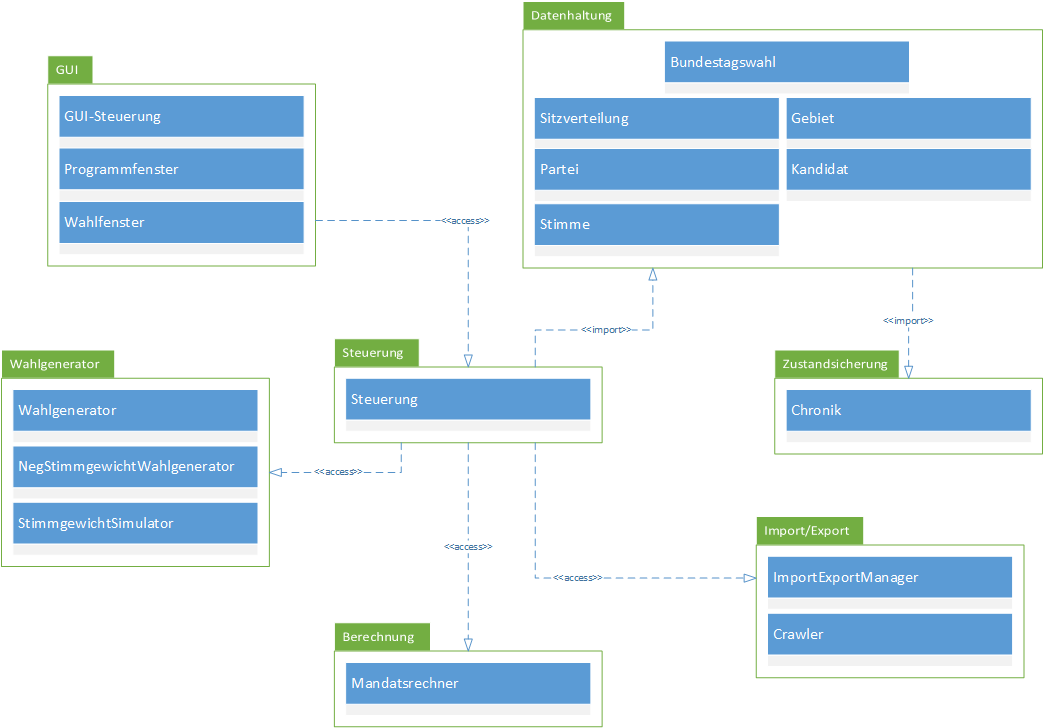
\includegraphics[scale=0.5]{Paketdiagramm} \caption{Paketdiagramm des Klassendiagramms}
\end{figure}
\newpage
\section{Klassendiagramm}
\subsection{GUI}
\begin{figure}[!ht]
\centering
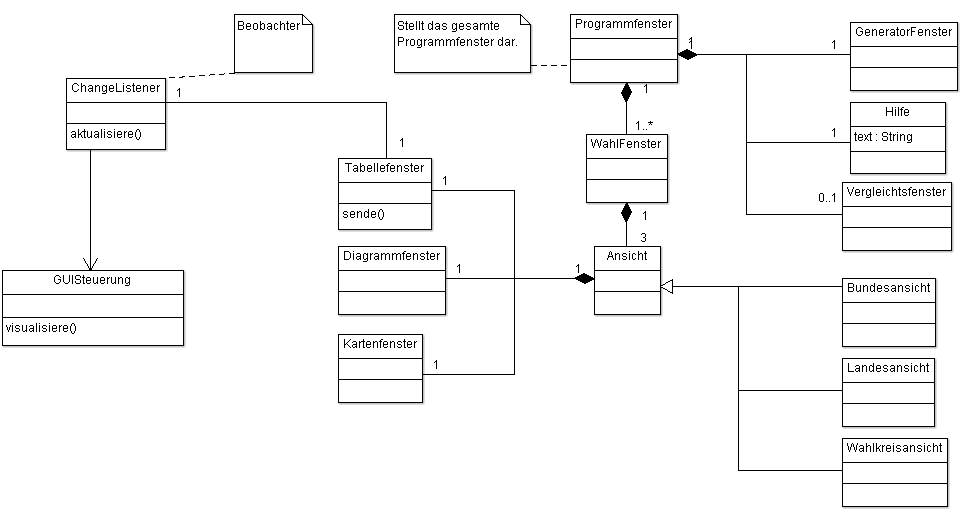
\includegraphics[scale=0.55]{GUI-Abschnitt.png} \caption{GUI Komponente} 
\end{figure}

Zum GUI-Teil gehören alle Klassen, die dazu beitragen, das Datenmodell bestmöglich auf der grafischen Benutzeroberfläche darzustellen. Im folgenden werden wichtige Klasse der GUI erläutert.


\begin{description}

\item  {\myma{{ProgrammFenster}}} \\
Das {\myma{ProgrammFenster}} repräsentiert das gesamte Programm auf der grafischen Benutzeroberfläche.
	\begin{description}
		\item {\mymo{{wechsleTab(w : WahlFenster)}}} \\
		Diese Funktion wird beim Wechsel von Tabs aufgerufen. Dabei wird in der Steuerung das Attribut ```aktuelleBTW'' verändert auf die zu w zugeordnete Bundestagswahl. Dies führt dazu, dass einige Funktionen in {\myma{Steuerung}} wie {\mymo{setzeZurueck()}} ohne zusätzliche Parameter mit der Bundestagswahl des aktuell offenen Tabs arbeiten.
	\end{description}

\item  {\myma{{VergleichsFenster}}} \\
Das {\myma{VergleichsFenster}} stellt zwei {\myma{Bundestagswahl}}-Objekte in einem Fenster nebeneinander dar, sodass beide direkt vergleicht werden können.
	\begin{description}
	\item {\mymo{zeigeVergleich()}} \\
	
	\item {\mymo{erstelleDiagramm()}} \\
	Erzeugt Diagramme unter den beiden Bundestagswahlen, welche die Sitzverteilungen anzeigen.
	\end{description}

\item  {\myma{{WahlFenster}}} \\
Das {\myma{WahlFenster}} repräsentiert eine einzelne {\myma{Bundestagswahl}}. In einem {\myma{ProgrammFenster}} sind mehrere {\myma{WahlFenster}} möglich, die in Form von Tabs dargestellt werden.
	\begin{description}
	\item {\mymo{{wechsleAnsicht(a : Ansicht)}}} \\
	Wechselt die Ansicht in eine andere gewünschte Ansicht.
	\item {\mymo{{bundestagswahlDarstellen(btw : Bundestagswahl)}}} \\
	Verteilt den drei Ansichten die Arbeit, das {\myma{Bundeswahl}}-Objekt darzustellen.
	\end{description} 

\item  {\myma{{Ansicht}}} \\
Die {\myma{Ansicht}} ist eine abstrakte Klasse. Diese kann drei Arten von Ansichten sein, {\myma{Bundes-}} {\myma{Landes-}} und {\myma{Wahlkreisansicht}}. Diese werden im Folgenden nicht näher erläutert.
	\begin{description}
	\item {\mymo{{zeigeKomponenten(btw : Bundestagswahl)}}} \\
	In jeder der drei Ansichten wird die Darstellung, des Bundestagswahl-Objekts auf die drei Fenster aufgeteilt. \\
	\end{description}

\item  {\myma{{TabellenFenster}}} \\
Das {\myma{TabellenFenster}} korrespondiert zu dem im Pflichtenheft beschriebenen Tabellenfenster. Es stellt Teile der {\myma{Bundestagswahl}}-Klasse dar.
	\begin{description}
	\item {\mymo{{tabellenFuellen(btw : Bundestagswahl)}}} \\
	Füllt das TabellenFenster mit den notwendigen Daten des Bundeswahl-Objekts.
	\end{description}

\item  {\myma{{DiagrammFenster}}} \\
Das {\myma{DiagrammFenster}} korrespondiert zu dem im Pflichtenheft beschriebenen Diagrammfenster. Je nach {\myma{Ansicht}} wird dort die {\myma{Sitzverteilung}}, prozentuale Anzahl der {\myma{Zweit-}} oder {\myma{Erststimmen}} angezeigt. 
	\begin{description}
	\item {\mymo{{erstelleDiagramm(btw : Bundestagswahl)}}} \\
	Erstellt ein Diagramm auf Grund der Daten der Bundestagswahl btw.
	\item {\mymo{{zeigeSitzverteilung()}}} \\
	Öffnet ein BerichtsFenster, in dem die Sitze der Verteilung näher erläutert werden.
	\end{description}

\item  {\myma{{KartenFenster}}} \\
Das {\myma{KartenFenster}} korrespondiert zu dem im Pflichtenheft beschriebenen Kartenfenster. Hier wird eine Liste der {\myma{Bundesländ}}er und {\myma{Wahlkreise}} und, wenn möglich, eine kartografische Darstellung {\myma{Deutschland}}s aus einem {\myma{Bundestagswahl}}-Objekt dargestellt.
	\begin{description}
	\item {\mymo{{zeigeInformationen(btw : Bundestagswahl)}}} \\
	Erstellt, wenn möglich, die kartografische Darstellung.
	\item {\mymo{{faerbeBundeslaender(btw : Bundestagswahl))}}} \\
	Färbt die einzelnen Bundesländer nach den Parteien, die die meisten Zweitstimmen haben. Diese Methode wird von zeigeInformationen benutzt.
	\end{description}

\item  {\myma{{GUISteuerung}}} \\
Die {\myma{GUISteuerung}} sorgt dafür, dass die aktuellste Version der {\myma{Bundestagswahl}} in einem {\myma{WahlFenster}} visualisiert wird. Dafür bekommt sie das aktuellste {\myma{Bundestagswahl}}-Objekt der {\myma{Steuerung}} und verteilt die Darstellungsarbeit an die Komponenten des {\myma{WahlFensters}}.
	\begin{description}
	\item {\mymo{{aktualisiereWahlfenster()}}} \\
	Diese Methode startet eine komplette Aktualisierung eines Wahlfensters. Hierbei werden auch alle Abhängigen Ansichten ebenfalls aktualisiert.
	\end{description}

\end{description}

\newpage
\subsection{Datenhaltung}
\begin{figure}[!ht]
\centering
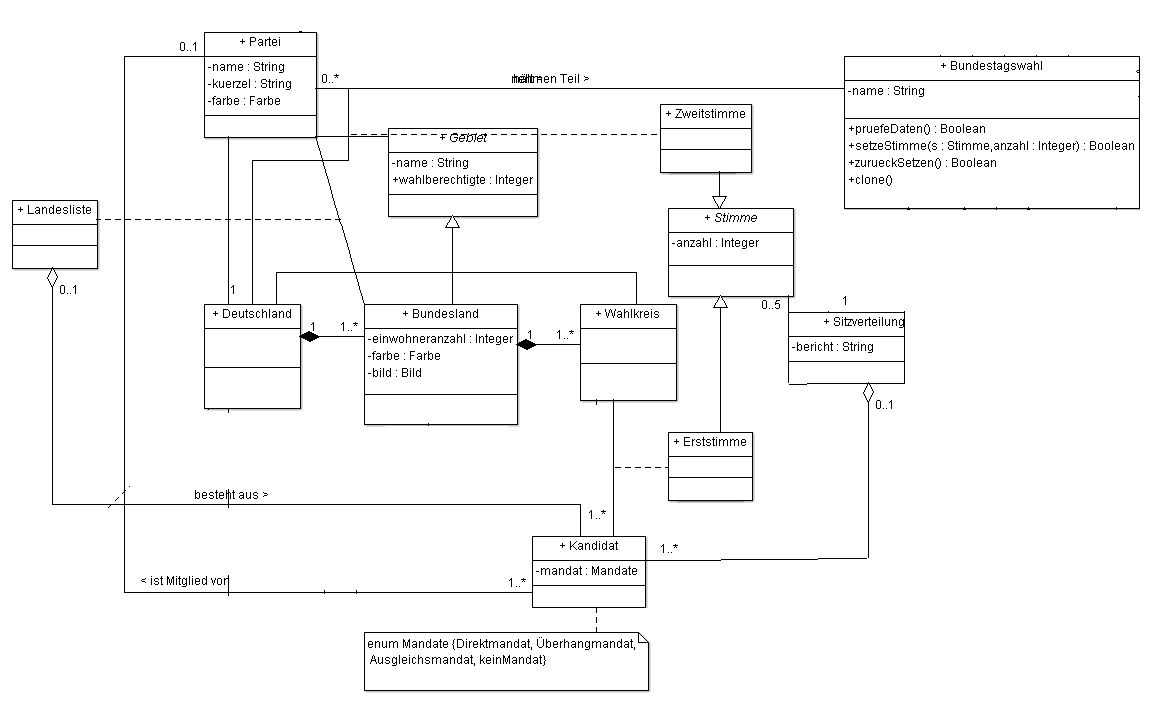
\includegraphics[scale=0.5]{Datenhaltung-Ausschnitt} \caption{Datenhaltungs Komponente} 
\end{figure}

Unter dem Datenmodell zählen alle Klassen, die Wahldaten oder die berechnete Sitzverteilung enthalten. Begründungen für Entwurfsentscheidungen und alle Klassen werden im folgenden aufgelistet:
\begin{description}

     \item {\myma{Bundestagswahl}} \\
     Eine Bundestagswahl stellt eine ganze Wahl dar. Es hat einen Namen wie "Bundestagswahl 2013". Dieser Name wird als Titel in der GUI auf dem betroffenen Tab angezeigt. Jede Bundestagswahl besitzt aufgrund der änderbaren Parteien pro Bundestagswahl eine eigene Liste an {\myma{Partei}}-Objekten. Des weiteren gibt es ein {\myma{Sitzverteilung}}-Objekt. \\
Folgende Methoden sind enthalten:
          \begin{description}
               \item {\mymo{prüfeDaten()}}\\
               Überprüft, ob die eingegebenen Stimmen gültig sind und unterzieht diese einem Konsistenz-Test. Die Methode wird nach jeder Stimmveränderung ausgeführt. Falls der Test nach einer Stimmveränderung fehlschlägt, wird die Stimme mithilfe der {\myma{Chronik}} zurückgesetzt und eine Fehlermeldung ausgegeben.

              \item {\mymo{setzeStimme(s:Stimme,anzahl:Integer) : Boolean}}\\
               Wird von der GUI über die Steuerung aufgerufen. Es wird das zu verändernde {\myma{Stimme}}-Objekt und die neue Anzahl der Stimmen übergeben. Es findet eine Vorüberprüfung statt, in der ermittelt wird was genau verändert wird. Es dürfen Erststimmen nur auf Wahlkreisebene und Zweitstimmen auf Wahlkreis-, Landes- und Bundesebene verändert werden. Die zu verändernde {\myma{Stimme}} wird geklont und in der {\myma{Chronik}} gespeichert. Dabei können drei Fälle auftreten: \\
               Falls die assoziierte Klasse von  {\myma{Stimme}}:\\
               ... ein {\myma{Wahlkreis}}-Objekt ist, wird der enthaltene Wert ``anzahl'' verändert in den Wert des übergebenen Parameters ``anzahl''. \\
               ... ein {\myma{Bundesland}}-Objekt ist, wird die Differenz der anzahl an Stimmen auf alle Wahlkreise des betroffenen Bundeslandes iterativ hinzugefügt oder abgezogen. \\
               ... ein {\myma{Deutschland}}-Objekt ist, wird die Differenz der Anzahl an Stimmen auf alle Wahlkreise der Bundesländer iterativ hinzugefügt oder abgezogen.\\
Zum Schluss wird die Methode {\mymo{prüfeDaten()}} aufgerufen.
               
               \item {\mymo{zurueckSetzen() : Boolean}}\\
               Ruft die Methode {\mymo{restauriereStimme()}} in der {\myma{Chronik}} auf und setzt eine {\myma{Stimme}} zurück. Es wird dabei die Methode {\mymo{setzeStimme(s:Stimme, anzahl:Integer)}} verwendet um die Stimmen zu ändern. Falls das Rücksetzen fehlschlägt ist der Rückgabewert ``false''. Andernfalls wird erneut {\mymo{restauriereStimme()}} aufgerufen um den neu erstellten Chronik-Eintrag in{\mymo{setzeStimme(s:Stimme, anzahl:Integer)}} zu entfernen. Anschließend wird ``true'' zurückgegeben.
               
               \item {\mymo{clone() : Bundestagswahl}}\\
               Macht eine ``deep copy'' von der aktuellen Bundestagswahl und gibt dies zurück.
          \end{description}

     \item {\myma{Partei}} \\
     Ein Objekt dieser Klasse spiegelt eine vertretene Partei des Bundestages wieder. Jede Partei besitzt einen Namen, ein Kürzel und eine Farbe. Die Farbe wird verwendet, um in der kartografischen Ansicht die Bundesländer mit der Partei einzufärben, die in diesem Bundesland die meisten Zweitstimmen hat.

     \item {\myma{Gebiet}} \\
     Eine Abstrakte Klasse, die ein Gebiet darstellt. Es erbt den Klassen {\myma{Deutschland}}, {\myma{Bundesland}} und {\myma{Wahlkreis}}. Gebiet besitzt eine Assoziationsklasse ({\myma{Zweitstimme}}) mit {\myma{Partei}}. Jedes Gebiet besitzt einen Namen und ein Wert mit der Anzahl der Wahlberechtigten.

     \item {\myma{Deutschland}} \\
     {\myma{Deutschland}} besitzt eine Liste an {\myma{Bundesland}}-Objekten, die in der Wahl benutzt wurden. Diese Klasse wird beispielsweise verwendet, wenn die Zweitstimmen einer Partei in der {\myma{Bundesansicht}} verändert wurde. 

     \item {\myma{Bundesland}} \\
     {\myma{Bundeland}} besitzt eine Liste an {\myma{Wahlkreis}}-Objekten, die in der Wahl benutzt wurden. Diese Klasse wird beispielsweise verwendet, wenn die Zweitstimmen einer Partei in der {\myma{Landesansicht}} verändert wurde. Diese Klasse enthält zusätzlich einige weitere Attribute. Diese sind Einwohnerzahl (zur Berechnung der möglichen Anzahl der Sitze pro Bundesland), sitze (berechnete Anzahl der möglichen Sitze), Farbe (Farbe der Partei mit den meisten Zweitstimmen, wird im Mandatsrechner ausgemacht) und Bild um das Wappen des Bundeslandes zu Speichern. Der Wappen wird in der Landesansicht angezeigt.

     \item {\myma{Wahlkreis}} \\
	Ein {\myma{Wahlkreis}} besitzt zusammen mit {\myma{Kandidat}} eine Assotiationsklasse {\myma{Erststimme}}, was die Erststimme pro Wahlkreis und Kandidat/Partei wiederspiegelt. In der {\myma{Wahlkreisansicht}} werden Objekte dieser Klasse von einem spezifischen Bundesland dargestellt.
	
     \item {\myma{Stimme}} \\
	Dies ist eine Abstrakte Klasse, die eine Oberklasse von {\myma{Erststimme}} und {\myma{Zweitstimme}} ist. Diese Klasse wird bei Stimmveränderungen verwendet um ausmachen zu können, welche Stimme genau verändert wurde.
	
     \item {\myma{Erststimme}} \\
    Darf nur als Assoziationsklasse zwischen {\myma{Wahlkreis}} und ein {\myma{Kandidat}} existieren. Dies stellt sicher, dass die Erststimme einzig auf Wahlkreisebene verändert werden kann/darf. Der Grund für diese Entscheidung ist, die Komplexität bei Veränderung der Erststimmen auf Bundes- und Landesebene zu vermeiden.
    
     \item {\myma{Zweitstimme}} \\
	Eine Assoziationsklasse zwischen {\myma{Partei}} und {\myma{Gebiet}}. Ermöglicht die Veränderung der Zweitstimmen auf Bundes- Landes- als auch Wahlkreisebene.
	
     \item {\myma{Kandidat}} \\
	Ein Kandidat kann entweder Direktmandat, Überhandmandat, Ausgleichsmandat oder überhaupt kein Mandat sein. Des weiteren kann ein Kandidat Abgeordneter sein, falls dieser ein Attribut einer {\myma{Sitzverteilung}} besitzt.
	
     \item {\myma{Landesliste}} \\
	Die Assoziationsklasse zwischen {\myma{Partei}} und {\myma{Bundesland}}. Beinhaltet eine Liste an Kandidaten. Die Reihenfolge der Kandidaten ist hierbei entscheidend, da dies entscheidet welche Kandidaten als erstes ein Sitz zugeordnet wird.
	
     \item {\myma{Sitzverteilung}} \\
	In dieser Klasse wird ein Bericht angelegt, dass zeigen soll, welcher Sitz wie entstanden, und welcher Partei zugeordnet ist. Es enthält eine Liste an Kandidaten. \\
	Die Informationen werden mit dem {\myma{Mandatsrechner}} generiert. Es wird hierbei zwischen Direktmandaten, Überhangmandaten und Ausgleichsmandaten unterschieden. Die Informationen werden in {\myma{BerichtsFenster}} visualisiert.
\end{description} 


\newpage
\subsection{Steuerung}
\begin{figure}[!ht]
\centering
\includegraphics[scale=0.9]{Steuerung} \caption{Steuerung Komponente} 
\end{figure}
Die {\myma{Steuerung}} verbindet die unterschiedlichen Kompententen (GUI, Datenmodelle, etc.). Es wurde deshalb das Entwurfsmuster Fassade für den Entwurf der Klasse genommen. Da es nur ein eindeutiges Objekt von der Klasse geben soll, wird zusätzlich Einzelstück als ein weiteres Entwurfsmuster genutzt. Die Steuerung hält für jeden Tab im {\myma{Programmfenster}} ein {\myma{Buntestagswahl}}-Objekt.
\begin{description}
     \item {\mymo{Steuerung()}} \\
     Der private Konstruktor wird für das Entwurfsmuster Einzelstück gebraucht. Dadurch ist es nicht möglich eine neue Instanz von der Klasse zu erstellen.
     \item {\mymo{getInstance() : Steuerung}} \\
     Diese Methode gehört ebenfalls zum Entwurfsmuster Einzelstück, da das private Attribut nur als Rückgabewert einer Methode übergeben werden kann.
     \item {\mymo{importieren(csvDatei : Datei)}} \\
     Die in der GUI ausgewählte Datei wird an den {\myma{ImportExportManager}} gesendet. Wenn die Formatierung und der Inhalt der Datei stimmen, wird das übergebene {\myma{Bundestagswahl}}-Objekt gespeichert.
     \item {\mymo{exportieren(pfad : String)}} \\
     Es wird ein {\myma{Bundestagswahl}}-Objekt und ein Dateipfad an den {\myma{ImportExportManager}} gesendet, damit die Klasse eine CSV-Datei erstellt und diese speichert.
     \item {\mymo{berechneSitzverteilung() : Bundestagswahl}} \\
     Das aktuelle {\myma{Bundestagswahl}}-Objekt wird im passenden Mandatsrechner ausgewertet. Das Ergebnis wird als Rückgabewert von der {\myma{Steuerung}} zurückgegeben.
     \item {\mymo{zufälligeWahlgenerierung(anteile : Stimmanteile) : Bundestagswahl}} \\
     Es wird mit Hilfe des {\myma{Wahlgenerators}} und der {\myma{Stimmenanteile}} eine {\myma{Bundestagswahl}} erstellt und zurückgegeben.
     \item {\mymo{negStimmgewichtGenerierung(anteile : Stimmanteile)}}\\
     \item {\mymo{aktualisiereDaten(stimme : Stimme, anzahl : Integer)}} \\
     Die Methode speichert den alten Wert in der Chronik und kopiert den neuen Wert über Deep copy in die Daten.
     \item {\mymo{vergleicheWahlen(btw1 : Bundestagswahl, btw2 : Bundestagswahl)}} \\
     Es werden zwei Wahlen an das {\myma{Wahlvergleich}}-Objekt gesendet.
     \item {\mymo{zurueckSetzen() : Boolean}} \\
     Der aktuellen Stand des Programmes wird mit dem alten Stand ersetzt. Bei einer erfolgreichen Zurücksetzten ist der Rückgabewert der Methode true;
\end{description} 

\newpage
\subsection{Import/ Export}
\begin{figure}[!ht]
\centering
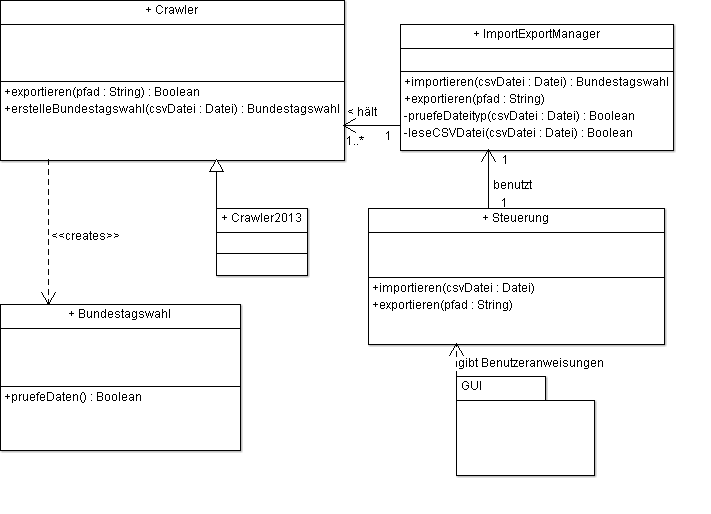
\includegraphics[scale=0.7]{Import-Export_Ausschnitt} \caption{Import/Export Komponente} 
\end{figure}


Hier sieht man den Aufbau des Import- bzw. Exportmoduls. Zur Übersichtlichkeit werden die zum Importieren/Exportieren nicht notwendigen Methoden in {\myma{Steuerung}} und die genaue Struktur hinter {\myma{Bundestagswahl}} und der GUI ausgeblendet. \\
Mit dem Programm wird nur ein vorimplementierter Crawler mitgegeben, der .csv-Dateien, die dem Format der .csv-Datei zur Bundestagswahl 2013 der Bundeswahlleiter-Webseite entsprechen, auswerten kann - dies ist {\myma{Crawler2013}}. Um jedoch die Möglichkeit zu garantieren, nachträglich weitere Crawler hinzuzufügen, haben wir uns dafür entschieden, eine abstrakte Oberklasse {\myma{Crawler}} zu verwenden, von der {\myma{Crawler2013}} erbt, und alle vorhandenen Crawler von der Klasse {\myma{ImportExportManager}} halten zu lassen. \\ Ausgelöst wird der ganze Import- bzw. Exportvorgang durch eine Benutzerinteraktion (z.B. Betätigen des Laden- Knopfs im Menü), worauf {\myma{Steuerung}} die entsprechenden Methoden von {\myma{ImportExportManager}} ausführt.

\subparagraph{Methoden}
\begin{description}
\item{\myma{ImportExportManager}}
\item {\mymo{importieren(csvDatei : Datei) : Bundestagswahl}} \\
Diese öffentliche Methode führt zuerst die private Methode {\mymo{pruefeDateityp()}} aus. Wenn diese true zurückgibt, wird die ebenfalls private Methode {\mymo{leseCSVDatei()}} ausgeführt. Wurde nun eine gültige Bundestagswahl zurückgegeben, wird diese an die Steuerung zurückgegeben, andernfalls ein Fehler ausgegeben.

\item {\mymo{pruefeDateityp(csvDatei : Datei) : Boolean}} \\
Prüft, ob es sich bei der gegebenen Datei um eine .csv-Datei handelt. Wenn dies der Fall ist, wird true zurückgegeben, andernfalls false.

\item {\mymo{leseCSVDatei(csvDatei : String) : Boolean}} \\
Durchläuft die Crawler-Liste und lässt die darin enthaltenen Crawler nacheinander versuchen, die .csv-Datei auszuwerten und mit den gewonnenen Informationen eine Bundestagswahl zu erstellen und zu füllen. Gelingt es einem Crawler, wird der Durchlauf abgebrochen und true zurückgegeben. 

\item{\myma{Crawler}}\\
\item {\mymo{exportieren(Pfad : String) : Boolean}} \\
Nimmt die aktuelle Bundestagswahl der Steuerung und schreibt die zugehörigen Wahldaten, ohne die berechneten Daten, in eine dem Pfad entsprechende .csv-Datei, deren Format Crawler bestimmt wird. Bei einem auftretenden Fehler wird false zurückgegeben.

\item {\mymo{erstelleBundestagswahl(csvDatei : Datei) : Bundestagswahl}} \\
Erstellt anhand einer .csv-Datei eine neue Bundestagswahl und versucht sie zu füllen. Wenn nicht alle nötigen Daten vorhanden sind, oder die Struktur der .csv-Datei nicht der vom Crawler geforderten Struktur entspricht, wird ein Fehler ausgegeben und der Import abgebrochen.
\end{description}

\newpage
\subsection{Wahlgenerierung}
\begin{figure}[!ht]
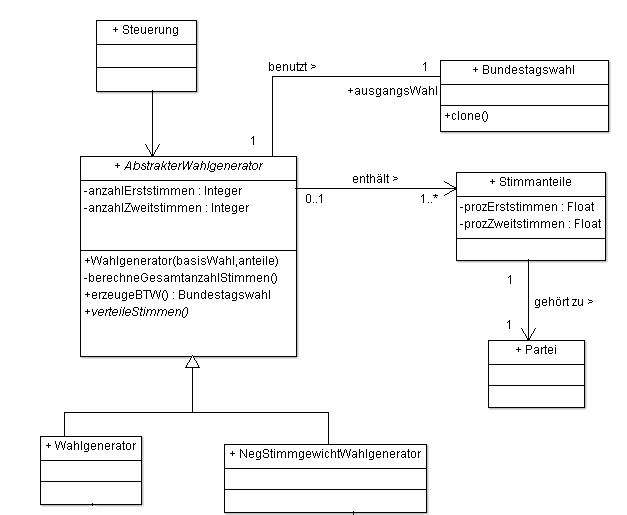
\includegraphics[scale=1.0]{Klassendiagramme/Wahlgenerator_Klassendiagramm.png} \caption{Wahlgenerierungs-Komponente} 
\end{figure}
Der obige Ausschnitt des Klassendiagramms zeigt das Wahldatengenerierungs-Modul.\\\\
Zur Übersichtlichkeit werden in den Klassen {\myma{Partei}}, {\myma{Steuerung}} und {\myma{Bundestagswahl}} nur die für dieses Modul relevanten Informationen angezeigt.\\\\
Mit diesem Modul können {\myma{Bundestagswahl}} Objekte anhand vorher definierten {\myma{Stimmanteilen}} auf Bundesebene generiert werden. Bei {\myma{Stimmanteile}} handelt es sich um eine Liste aller Parteien mit prozentualen Anteilen der Erst- und Zweitstimmen auf Bundesebene. Des weiteren benötigt der Wahlgenerator eine {\myma{basisWahl Bundestagswahl}} um Daten wie beispielsweise {\myma{Bundesländer}}, {\myma{Wahlkreise}} und {\myma{Wahlberechtigte}} zur Verfügung zu haben. Aus dieser basisWahl wird eine tiefe Kopie erstellt, deren Stimmzahlen anschließend verändert werden.\\\\

Neben dem {\mymo Wahlgenerator}, der alle Stimmen der jeweiligen Parteien zufällig auf Wahlkreise verteilt gibt es noch den {\mymo NegStimmgewichtWahlgenerator}. Dieser erzeugt Bundestagswahlen, die die Voraussetzungen erfüllen, welche für die Simulation des Negativen Stimmgewichts benötigt werden.\\

Dabei muss bei mindestens einer Partei der prozentuale Anteil ihrer relevanten Zweitstimmen größer als der prozentuale Anteil ihrer Mandate sein. Relevante Zweitstimmen sind all diejenigen Zweitstimmen, die auf Landeslisten abgegeben werden, die keine Überhangmandate erzielen.

\subparagraph{Methoden}
\begin{description}
\item {\mymo{Wahlgenerator(basisWahl : Bundestagswahl, anteile : Stimmanteile)}} \\
Der Konstruktor dieser Klasse. Wird verwendet um einen neuen {\mymo{Wahlgenerator}} zu erstellen. Hier werden die Attribute basisWahl, anteile, erststimmenAnzahl und zweitstimmenAnzahl gesetzt.
\item {\mymo{berechneGesamtanzahlStimmen()}} \\
Diese Methode ist privat und wird von dem Konstruktor verwendet um die Attribute {\mymo{anzahlErststimmen}} und {\mymo{anzahlZweitstimmen}} zu berechen. Hierzu werden die Stimmanteile mithilfe der Anzahl aller Wahlberechtigten in absolute Zahlen für Erst- und Zweitstimmen umgerechnet.
\item {\mymo{erzeugeBTW() : Bundestagswahl}} \\
Erzeugt eine neue Bundestagswahl auf der Grundlage der basisWahl und füllt diese mit den Erst- und Zweitstimmen.
\item {\mymo{verteileStimmen()}} \\
Diese Methode verteilt alle Erst- und Zweitstimmen auf die Wahlkreise der Bundestagswahl. Diese Methode muss in jeder Unterklasse von Wahlgenerator implementiert werden.
\end{description}

\newpage
\subsection{Chronik}
\begin{figure}[!ht]
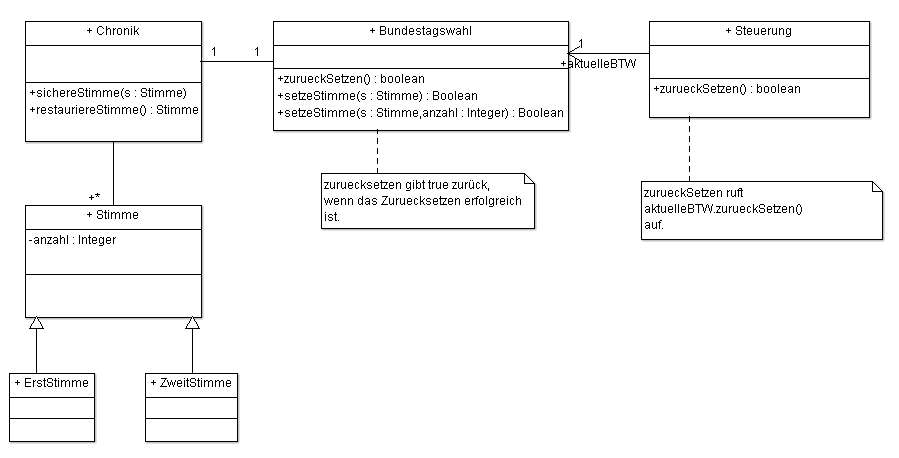
\includegraphics[scale=0.7]{Klassendiagramme/Chronik_Ausschnitt} \caption{Chronik-Komponente} 
\end{figure}

Die Klasse {\myma{Chronik}} gibt dem Programm die Funktionalität, Veränderungen an den Stimmen rückgängig zu machen. Jede {\myma{Bundestagswahl}} hat hierbei eine eigene Chronik. {\myma{Chronik}} wird in dem Konstruktor von {\myma{Bundestagswahl}} erzeugt, und ist daher in jedem {\myma{Bundestagswahl}}-Objekt enthalten. Es besitzt eine Menge von {\myma{Stimmen}}-Objekten. Bei jeder Veränderung wird ein neues {\myma{Stimmen}}-Objekt angelegt, was die Veränderung wiederspiegelt.
\
Die Methode {\myma{sichereStimme}} wird von dem {\myma{Bundestagswahl}}-Objekt bei jedem Aufruf von {\myma{setzeStimme}} aufgerufen.
\subparagraph{Methoden}
\begin{description}
\item {\mymo{sichereStimme(s : Stimme)}} \\
Diese Funktion wird von dem assoziierten {\myma{Bundestagswahl}}-Objekt innerhalb der {\mymo{setzeStimme}}-Funktion aufgerufen. Falls bereits fünf {\myma{Stimmen}}-Objekte vorhanden sind, wird das älteste entfernt.
\item {\mymo{restauriereStimme() : Stimme}} \\
Wird von der {\myma{Steuerung}} über die aktuelle Bundestagswahl mit der Funktion{\mymo{zurueckSetzen()}} aufgerufen und gibt die zuletzt hinzugefügte {\myma{Stimme}} zurück. Die Bundestagswahl ersetzt dann die aktuelle Stimme mit der restaurierten Stimme.
\end{description}

\newpage
\subsection{Mandatsrechner}
\begin{figure}[!ht]
\centering
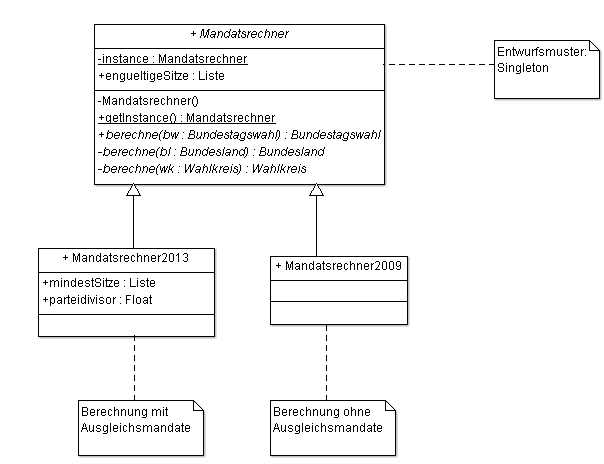
\includegraphics[scale=0.6]{Mandatsrechneralles.png} \caption{Mandatsrechner-Komponente} 
\end{figure}
Die Berechnung der Wahl wird mit Hilfe des {\myma{Mandatsrechners}} realisiert. Es stehen die Klasse \\{\myma{Mandatsrechner2013}}, die das Berechnungsverfahren von der Bundestagswahl 2013 benutzt und die Klasse {\myma{Mandatsrechner2009}}, die das Berechnungsverfahren von der Bundestagswahl 2009 benutzt zur Verfügung. Beide Klassen erben von der abstrakten Klasse {\myma{Mandatsrechner}}. Dadurch besteht die Möglichkeit, weitere Berechnungsverfahren in späteren Versionen zu dem Programm hinzuzufügen. Da nur ein Objekt von dem {\myma{Mandatsrechner}} gebraucht wird, wird das Entwurfsmuster Einzelstück eingesetzt. Deswegen hält die Klasse einen privaten Konstruktor. Die abstrakten Methoden {\mymo{berechne()}} werden überladen, damit sie durch ihre Eingabeparameter spezifiziert werden. Diese werden dann in den Unterklassen je nach Wahlgesetz angepasst. Neben der Berechnung wird ein Bericht über die Sitzverteilung erstellt, der zum Nachvollziehen der Sitzverteilung helfen soll.
\begin{large}
Methoden 
\end{large}
\begin{description}

\item {\mymo{berechne(wk: Wahlkreis):Wahlkreis}} \\
Es werden die Stimmen aus den jeweiligen Wahlkreis ausgewertet. Dabei wird der Wahlkreissieger bestimmt und die Anzahl der Zweitstimme von jeder Partei. Die Auswertung wird danach wieder in das Wahlkreis-Objekt geschrieben.
\item {\mymo{berechne(bl: Bundesland):Bundesland}} \\
Um das Bundesland zu berechnen, müssen vorher alle Wahlkreise berechnet werden. Deswegen werden alle Wahlkreise, die ein Bundesland hält, neu berechnet. Die Berechnung der einzelnen Bundesländer erfolgt parallel. Nachdem die berechneten Wahlkreise im Bundesland gespeichert wurden, wird das Bundesland berechnet. Hier wird das Verhältnis der Parteien im Bundesland berechnet, damit später klar ist wie viele Sitze eine Partei in diesem Bundesland bekommt. Diese Ergebnisse werden, wie beim Wahlkreis, im Bundeslandobjekt gespeichert und danach zurückgegeben. 
\item {\mymo{berechne(bw: Bundestagswahl):Bundestagswahl}} \\
Diese öffentliche Methode berechnet zuerst alle Bundesländer die sich in der Klasse befinden. Nachdem alle Bundesländer erfolgreich berechnet wurden, wird die endgültige Sitzverteilung nach dem jeweiligen Wahlgesetz berechnet. Die Sitzverteilung wird dann in dem Bundestagswahlobjekt gespeichert. Das Bundestagswahlobjekt wird danach wieder an die Steuerung zurückgegeben.
\item {\mymo{erstelleBericht(Zeile : String)}} \\
Während der Berechnung wird nebenbei eine Sitzverteilungsbericht verfasst, der beschreiben soll, wie die Sitzverteilung entstanden ist. Dabei wird die Methode immer aufgerufen, wenn eine Partei einen Sitz in der Sitzverteilung bekommen hat. Dies wird dann mit einer Zeile im Bericht protokolliert.
\end{description} 

\newpage
\subsection{Wahlvergleich}
\begin{figure}[!ht]
\centering
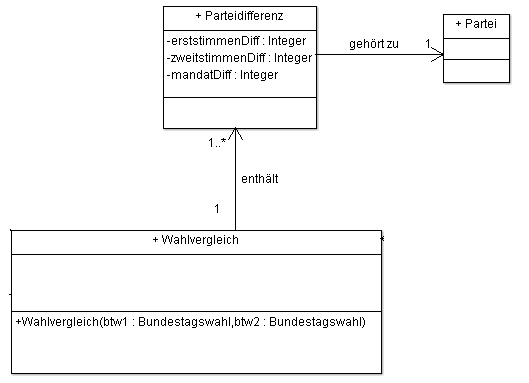
\includegraphics[scale=0.8]{Klassendiagramme/Wahlvergleich.png} \caption{Wahlvergleich-Modul} 
\end{figure}

Dieses Modul ermöglicht den Vergleich von zwei Bundestagswahlen.
Die Klasse {\myma{Wahlvergleich}} enthält zwei Bundestagswahlen sowie eine Liste aller relevanten Parteien mit den Differenzen von Erst-, Zweitstimmen sowie der Anzahl von Mandaten.

\subsection{Meldung}
\begin{figure}[!ht]
\centering
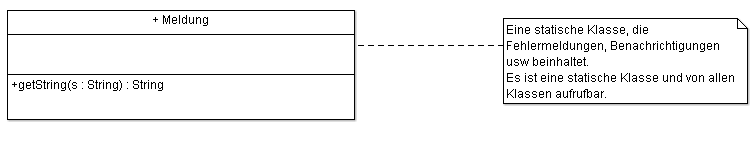
\includegraphics[scale=0.8]{Meldung_Ausschnitt.png} \caption{Meldungs-Klasse} 
\end{figure}
Die Klasse {\myma{Meldung}} ist verantwortlich für Fehlermeldungen, Benachrichtigungen und Fenstertexte. Es ist eine statische Klasse. Die Funktion {\mymo{getString}} gibt zu einem gegebenen Schlüssel ein String zurück. Die Strings dieser Klasse werden in einem externen Textdokument gelagert.

\newpage
\section{Sequenzdiagramme}
\subsubsection{Berechnung der Sitzverteilung}
\begin{figure}[!ht]
\centering
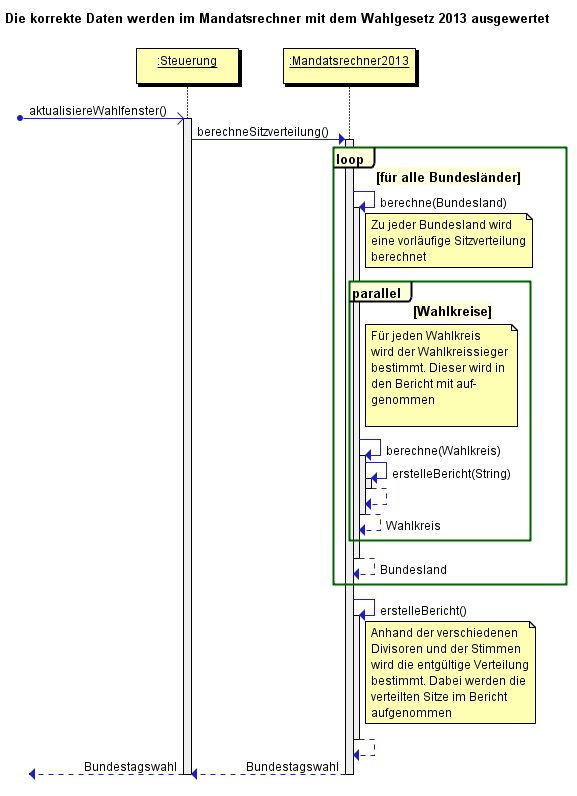
\includegraphics[scale=0.5]{berechne2013}\\ \caption{Sequenzdiagramm zur Stimmenänderung}
\end{figure}
Das {\myma{Bundestagswahl}}-Objekt wir mit dem {\myma{Mandatsrechner2013}} ausgewertet.  
\subsection{DeepCopy}
\begin{figure}[!ht]
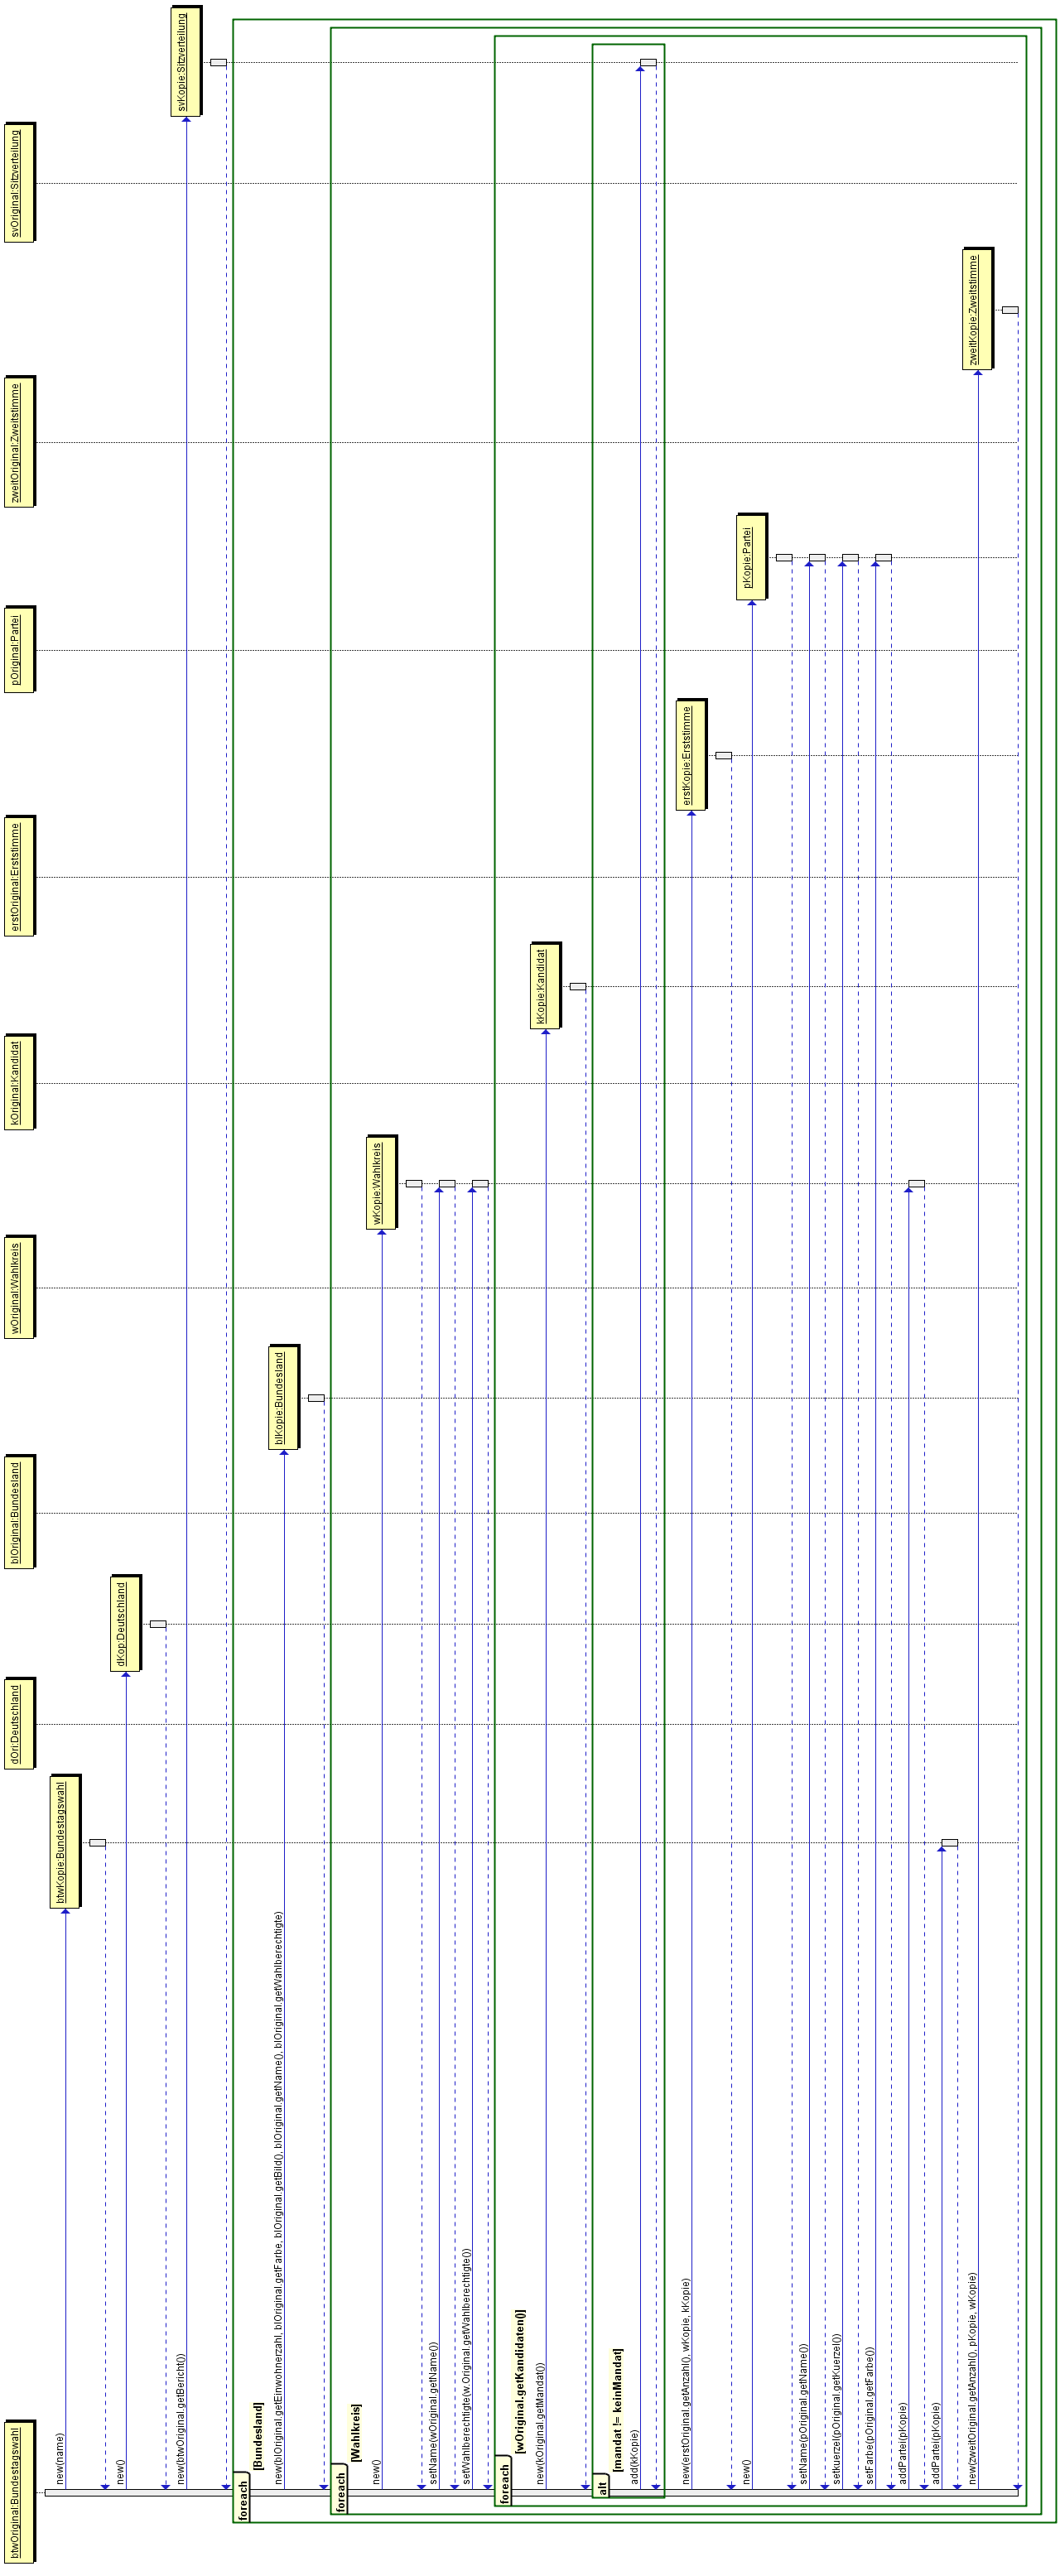
\includegraphics[scale=0.3]{DeepCopy.png} \caption{Kopieren einer Bundestagswahl} 
\end{figure}
\subsection{Import}
\begin{figure}[!ht]
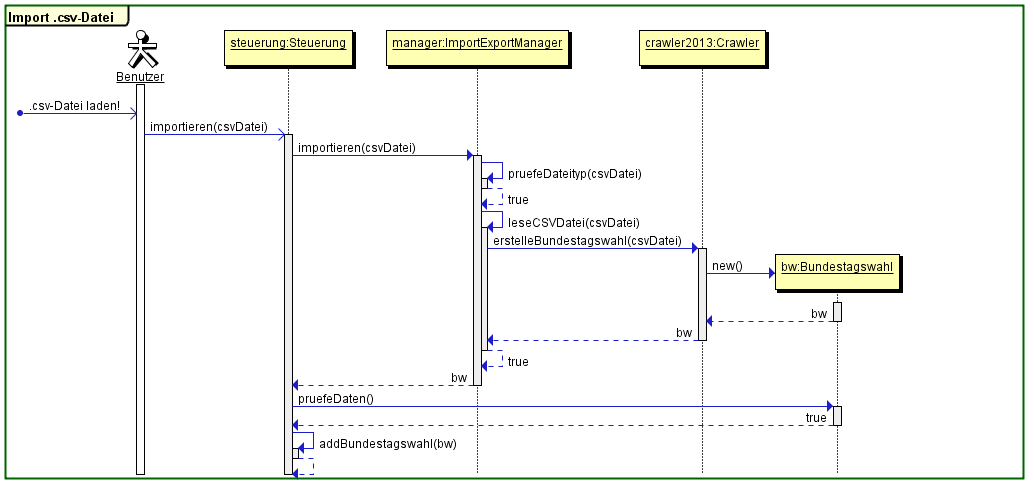
\includegraphics[scale=0.5]{Sequenzdiagramme/Import_Sequenzdiagramm.png} \caption{Import Sequenzdiagramm} 
\end{figure}
Hier wird eine gültige .csv-Datei, d.h. Format und Inhalt betreffend, importiert. Vorher wurde bereits ein Datei-Objekt csvDatei erstellt, das nun übergeben wird.

\newpage
\subsection{Wahlgenerierung}
\begin{figure}[!ht]
\centering
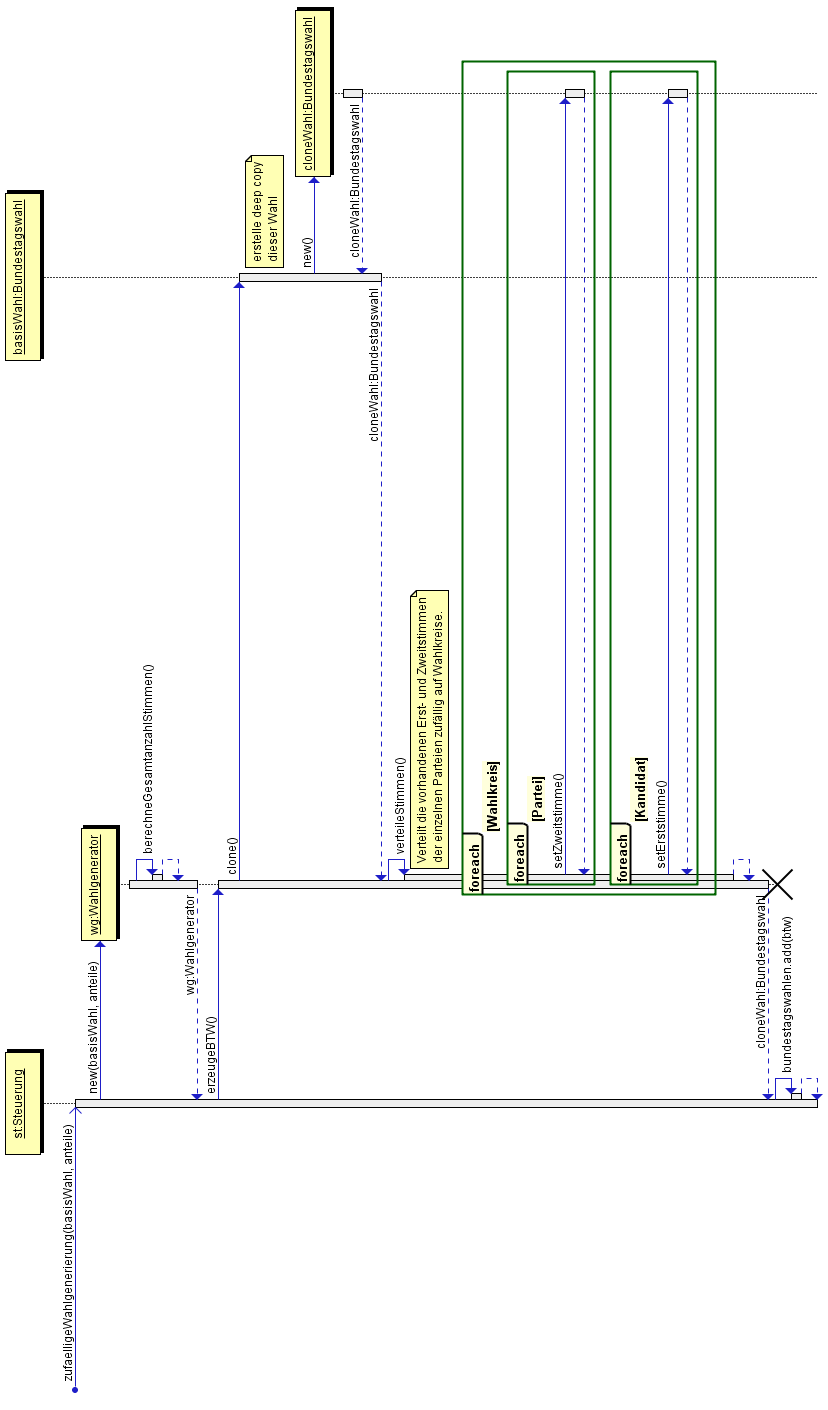
\includegraphics[scale=0.55]{Sequenzdiagramme/Wahlgenerierung.png} \caption{Sequenzdiagramm zur Wahlgenerierung}
\end{figure}
In der Methode {\mymo{zufaelligeWahlgenerierung(basisWahl : Bundestagswahl, anteile : Stimmanteile) : Bundestagswahl}} wird zuerst ein neuer Wahlgenerator erzeugt. In dem Konstruktor des Wahlgenerators werden die absoluten Stimmzahlen berechnet und alle Attribute gesetzt.\\
Anschließend wird von der Steuerung die Methode {\mymo{erzeugeBTW()}} ausgeführt. In dieser Methode wird zuerst eine tiefe Kopie der basisWahl erstellt. In dieser Kopie werden dann die Stimmen auf alle Wahlkreise verteilt. Die Erststimmen auf die Kandidaten und die Zweitstimmen auf die Parteien. Diese Wahl wird am Ende als Ergebnis der Methode berechneBTW() zurückgegeben und in der Steuerung in die Liste alle Bundestagswahlen eingefügt.

\newpage
\subsection{Paradoxe Wahlgenerierung und Vergleich}

\newpage
\subsection{Chronik}
\begin{itemize}
	\item Veränderung an den Stimmen \\
		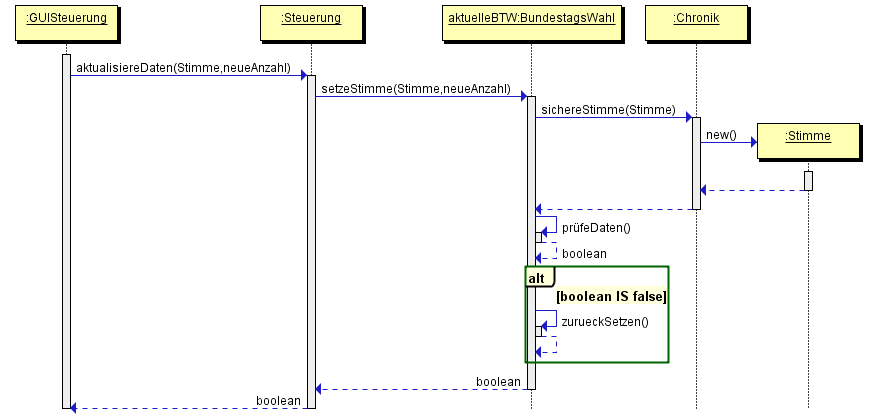
\includegraphics[scale=0.7]{Sequenzdiagramme/Chronik_Sequenzdiagramm-stimmenaendern.png}
	\item Restaurieren einer Stimme \\
		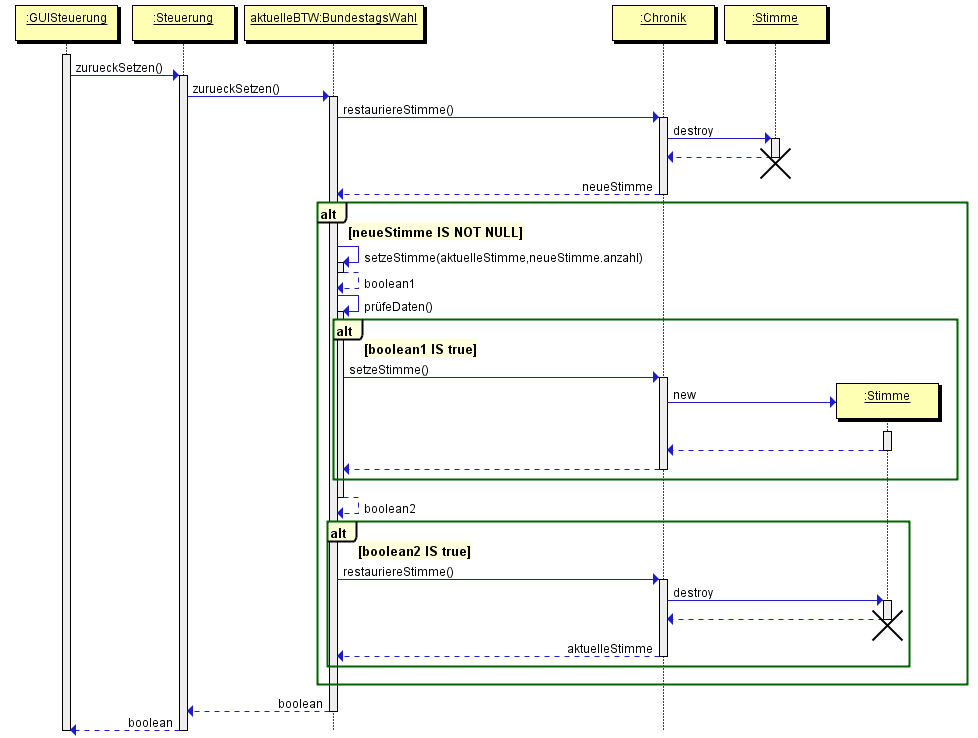
\includegraphics[scale=0.7]{Sequenzdiagramme/Chronik_Sequenzdiagramm-restaurieren.png}
		\\
		Stimmen werden in der Chronik werden Stack-artig zurückgegeben. Sobald eine Bundestagswahl rückgängig gemacht wurde, wird die neue Bundestagswahl als Rückgabewert zurückgegeben.
	\item Beispielszenario	
\end{itemize}
%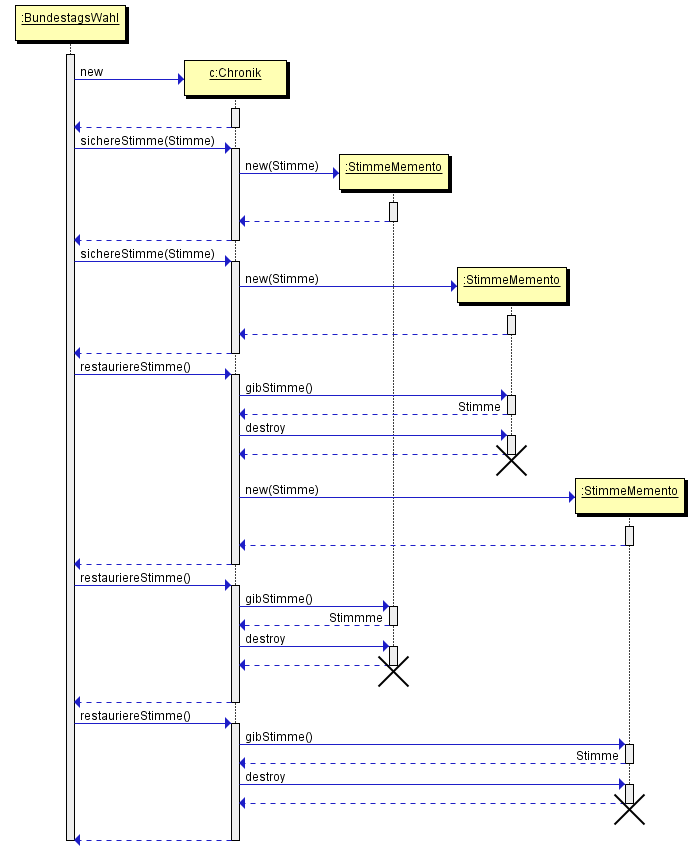
\includegraphics[scale=0.75]{Chronik_Sequenzdiagramm.png}

\newpage
\subsection{GUI}
\subsubsection{Aktualisierung}
Hier sieht man die Aktualisierung der grafischen Benutzeroberfläche. Eine neue Sitzverteilung wurde berechnet und in Form einer Bundestagswahl-Klasse in der Steuerung abgelegt. \\
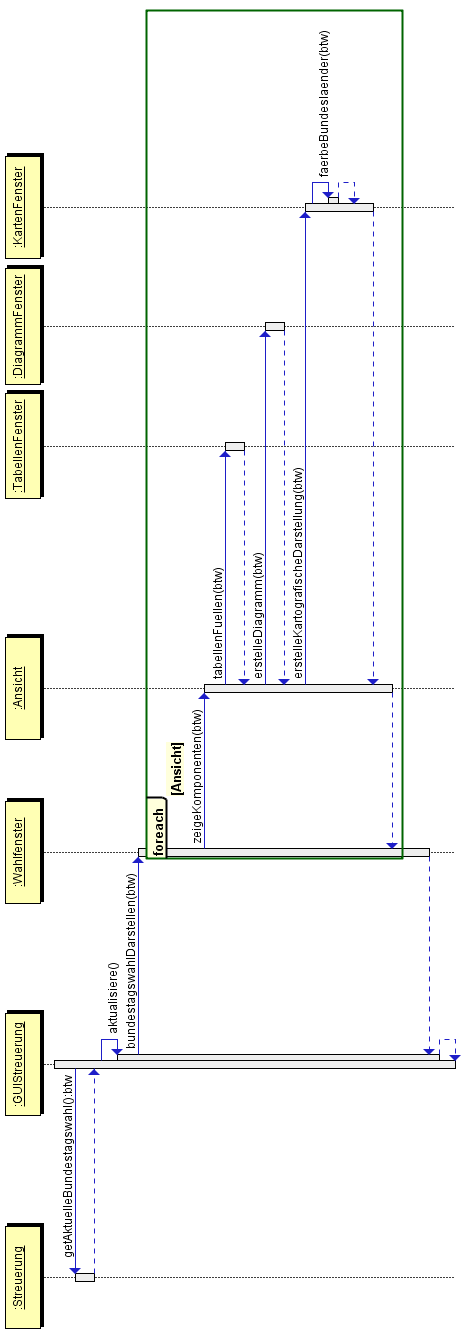
\includegraphics[scale=0.5]{GUI_Aktualisierung.png}

Die GUISteuerung aktualisiert ihr Bundeswahlobjekt, indem sie sich dieses von der Steuerung holt. Dann wird die Aktualisierung mit der Methode aktualisiereWahlfenster() gestartet. In dieser wird dem Wahlfenster Bundestagswahl übergeben und dieses verteilt die Visualisierung an die drei Ansicht. In diesen wird dann die Datendarstellung and die drei Fenster verteilt. In diesem Fall wird eine kartografische Ansicht erstellt, wodurch auch die private Methode faerbeBundeslaender() verwendet wird.

\newpage
\subsubsection{Stimmenänderung}
\begin{figure}
\centering
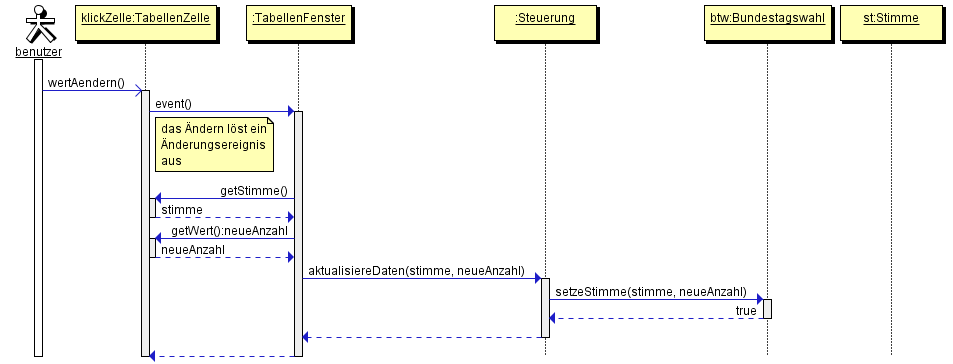
\includegraphics[scale=0.5]{GUI_Stimmenaenderung}\\ \caption{Sequenzdiagramm zur Stimmenänderung}
\end{figure}
Der Benutzer ändert eine beliebige Stimme im Tabellenfenster. Dadurch wird ein Ereignis ausgelöst, wodurch das
TabellenFenster reagiert. Es fragt die zur Tabellenzelle korrespondierende Stimme und den neuen Wert ab und übergibt
diese zwei Daten an die Steuerung. Die Steuerung ruft auf dem aktuellen Bundeswahl-Objekt die Methode setzeStimme()
mit den Parametern Stimme und der neuen Anzahl an Stimmen. Was dabei passiert siehe Chronik. Alles läuft gut ab, die alte Stimme wird in die Chronik aufgenommen und die alte Stimme in dem Bundestagswahl-Objekt durch die alte ersetzt.
\newpage
\section{Implementierungsphasen-Zeitplan}
\begin{figure}[!ht]
\centering
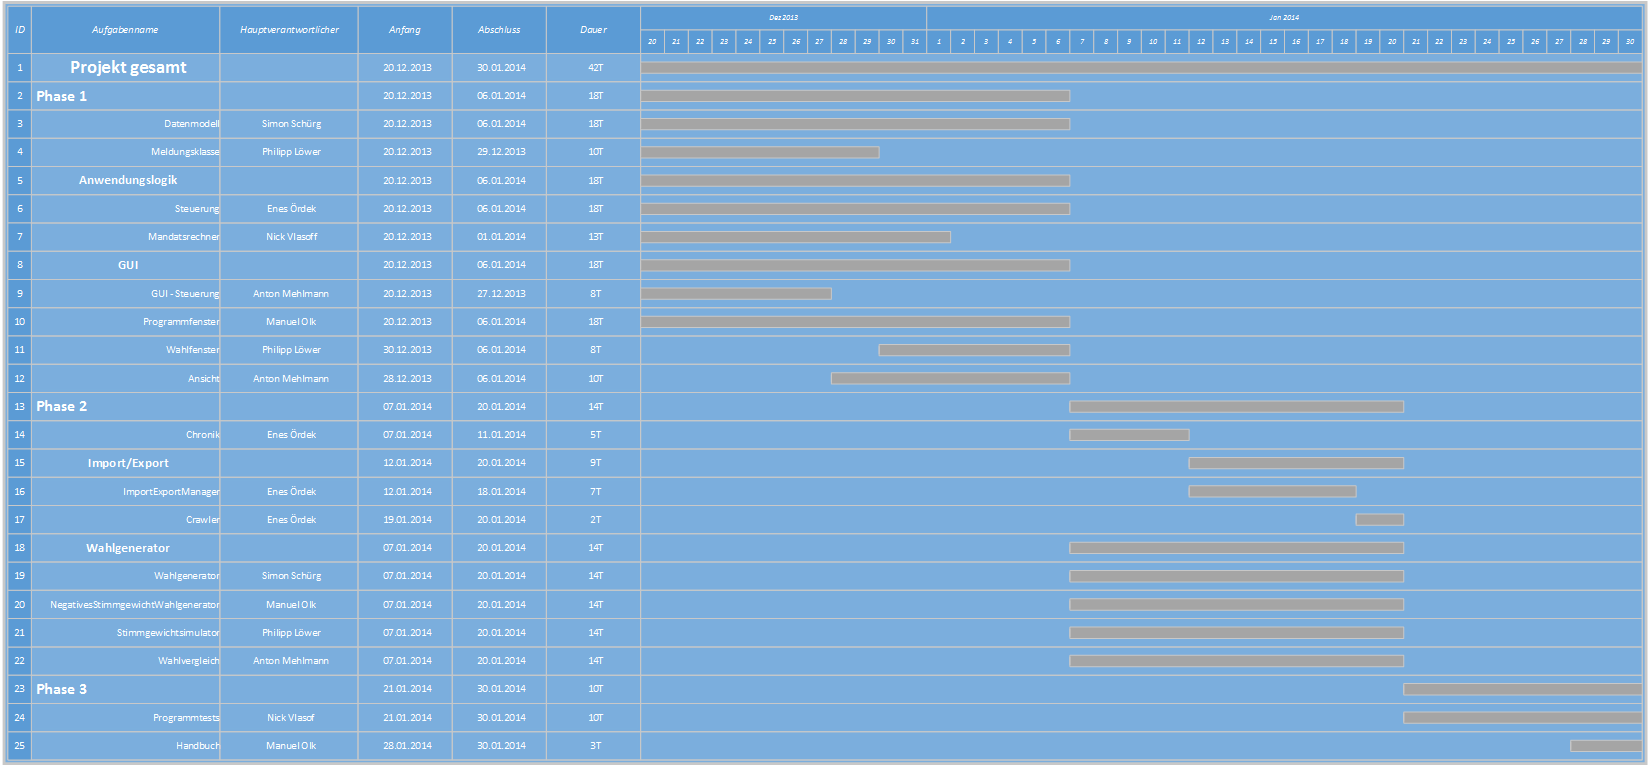
\includegraphics[angle=90, scale=0.45]{Gantt-Diagramm} \caption{Gantt-Diagramm zur Zeitplanung der Implementierungsphase}
\end{figure}


\begingroup
\parindent 0pt
\parskip 2ex
\def\enotesize{\normalsize}

\endgroup
\end{document}
